\documentclass[preprint,12pt]{elsarticle}

\usepackage{amsmath,amssymb,amsfonts,amsthm}
\usepackage{booktabs}
\usepackage{graphicx}
\usepackage{multirow}
\usepackage[table]{xcolor}
\usepackage{array}
\usepackage{caption}
\usepackage[T1]{fontenc}
\usepackage{microtype}
\usepackage{algorithm}
\usepackage{algpseudocode}
\usepackage[colorlinks=true,linkcolor=blue,citecolor=blue,urlcolor=blue]{hyperref}

\newcommand{\indicator}{\mathbf{1}}
\newcommand{\CCR}{\mathcal{L}_{\mathrm{CCR}}}
\newcommand{\CE}{\ell_{\mathrm{CE}}}
\newcommand{\tb}[1]{\textbf{#1}}
\newcommand{\scs}[1]{\scriptsize{$\pm$#1}}
\newcolumntype{C}[1]{>{\centering\arraybackslash}p{#1}}

\newtheorem{proposition}{Proposition}
\newtheorem{corollary}{Corollary}[proposition]
\newtheorem{remark}{Remark}
\newtheorem{definition}{Definition}
\newtheorem{hypothesis}{Hypothesis}

\journal{Neurocomputing}

\begin{document}

\begin{frontmatter}

\title{When Labels Lie and Classes Skew: Robust Tabular Deep Learning via Confidence-Calibrated Reweighting}

\author[aff1]{Md Shoaib Uddin Chanda}
\ead{mdshoaibuddinchanda@gmail.com}

\address[aff1]{Department of Computer Science and Engineering
  (Artificial Intelligence and Machine Learning),
  Lords Institute of Engineering and Technology,
  Hyderabad 500091, Telangana, India
  (Affiliated with Osmania University, Hyderabad).}

%% ------------------------------------------------------------------
\begin{abstract}
Deep neural networks on tabular data encounter compounding failure modes under concurrent class imbalance and asymmetric label noise. Standard loss functions treat mislabeled minority instances as hard examples and paradoxically amplify corrupted gradients, while existing noise-robust objectives overlook imbalance. In this paper, we establish that dynamic confidence-aware reweighting is the principal driver of noise robustness, while per-batch normalization ensures optimization stability. We formulate \emph{Confidence-Calibrated Reweighting} (CCR), an autograd-detached objective integrating confidence-inverse penalties, historical prediction variance gating, and static class weighting, paired with an invariant batch normalization operator that enforces a unit batch-mean weight. We prove an analytical supremum bound $\sup(S/B) \le 2.125$ and observe empirical weight deflation ($S/B \in [0.327, 1.022]$, $P_{99} \le 0.985$). Across a structured $10+2+2$ benchmark (10 Core binary, 2 multiclass, 2 clinical datasets) evaluated against 9 baseline losses and tree ensembles (XGBoost, LightGBM, CatBoost), CCR substantially mitigates degradation under severe 40\% asymmetric noise: it preserves minority recall at 0.6690 versus 0.5478 for Cross-Entropy (+12.12 percentage points / 22.1\% relative) and approximately 0.39--0.42 for tree ensembles (LightGBM 0.3897, CatBoost 0.4080, XGBoost 0.4156), while improving Macro-F1 by 4.86 percentage points (6.37\% relative) over Cross-Entropy with zero clean-data penalty (+0.15 percentage points). CCR outperforms dedicated noise-robust baselines, while static class-weighted objectives remain competitive in pure imbalance regimes. Mechanistic gradient attribution confirms CCR attenuates corrupted-sample gradient mass ($R_{\mathrm{noise}}$ by 15\%--25\%) and reduces gradient norm volatility by 10\%--35\%. Finally, architecture transferability experiments confirm consistent robustness gains across TabularMLP, TabularResNet, and FT-Transformer.
\end{abstract}

\begin{keyword}
tabular deep learning \sep label noise \sep class imbalance \sep dynamic sample reweighting \sep batch normalization \sep gradient scale invariance
\end{keyword}

\end{frontmatter}


%% ==================================================================
\section{Introduction}
\label{sec:intro}

Tabular data remains the foundation of high-stakes predictive systems across financial risk assessment, medical diagnosis, fraud detection, and industrial fault monitoring. In clean-data regimes with rotationally non-invariant feature structures, gradient-boosted decision trees (GBDTs) such as XGBoost~\cite{chen2016xgboost}, LightGBM~\cite{ke2017lightgbm}, and CatBoost~\cite{prokhorenkova2018catboost} have traditionally demonstrated superior empirical performance over deep neural networks~\cite{grinsztajn2022why,gorishniy2021revisiting}. However, production tabular environments routinely depart from clean benchmark conditions: training datasets frequently suffer from concurrent \emph{class imbalance} (where positive events are rare) and \emph{asymmetric label noise} (where ambiguous or rare positive cases are systematically misannotated as negative)~\cite{frenay2014classification,he2009learning}.

\begin{figure*}[htbp]
\centering
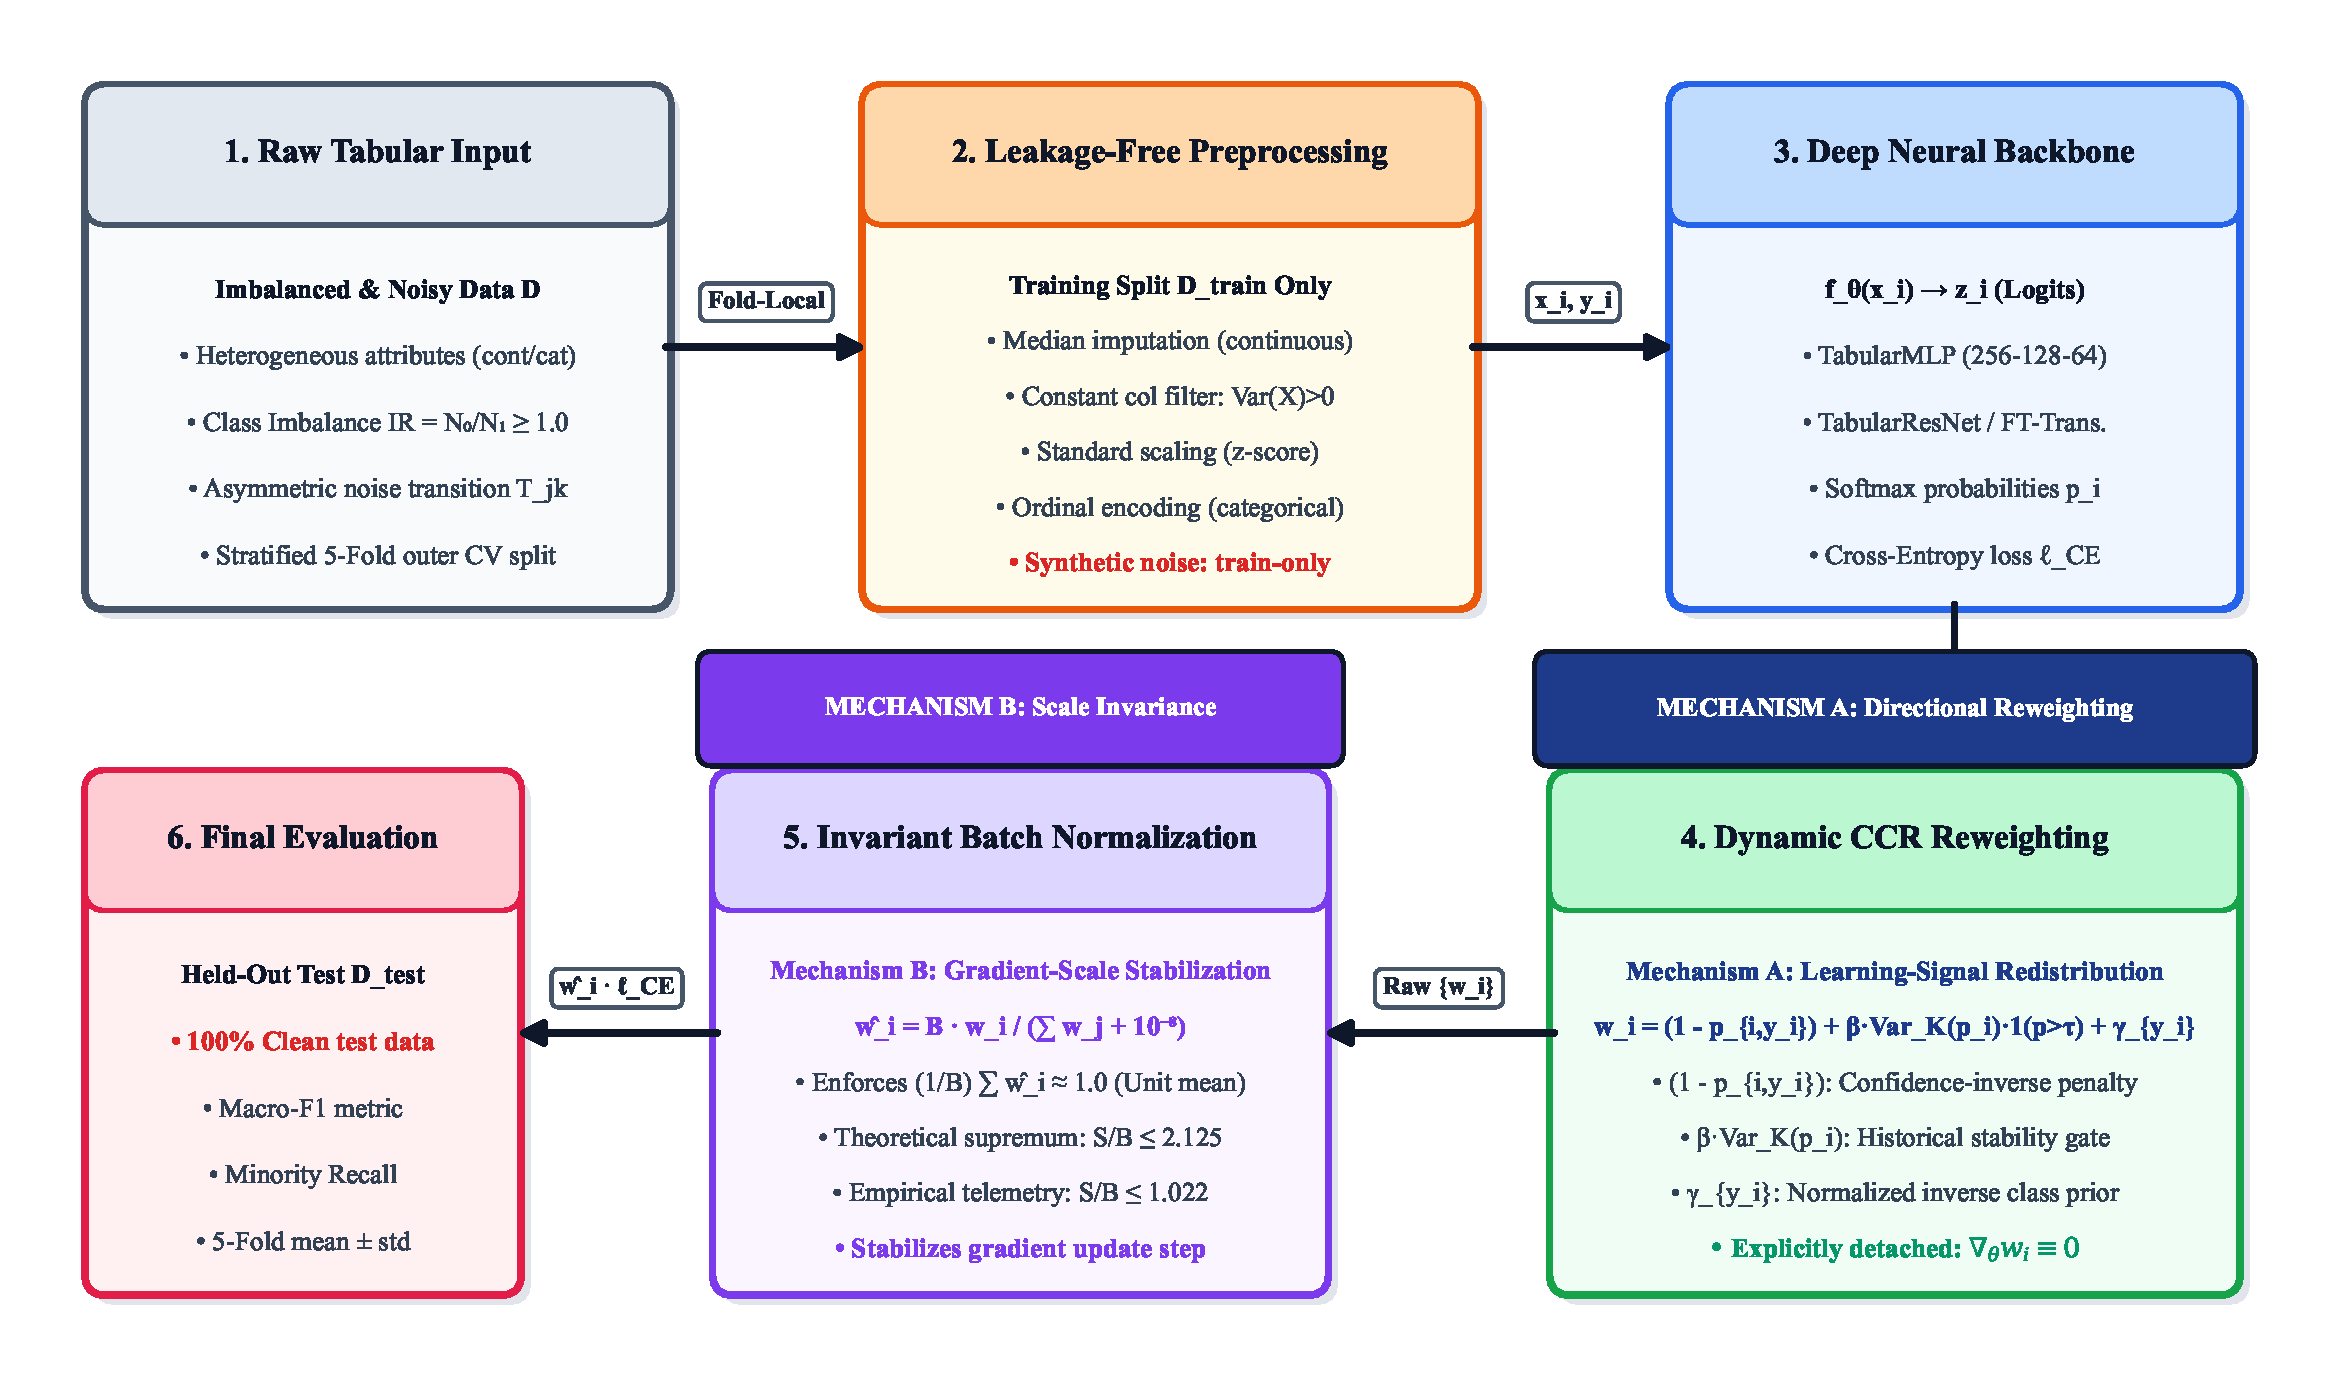
\includegraphics[width=\linewidth]{fig1_schematic.pdf}
\caption{Overview of the Confidence-Calibrated Reweighting (CCR) end-to-end training and evaluation framework. Raw tabular records undergo stratified 5-fold cross-validation and fold-local preprocessing with noise injected strictly on training splits. Dynamic weights are computed via confidence-inverse penalties, historical prediction variance, and class balance, detached from autograd, and normalized per-batch ($\frac{1}{B}\sum \hat{w}_i \approx 1.0$) to stabilize gradient updates prior to clean held-out evaluation.}
\label{fig:schematic}
\end{figure*}

\subsection{The Compounding Degradation of Imbalance and Asymmetric Noise}

When class imbalance and label noise co-occur, they trigger a compounding failure mode for standard classification objectives. Consider an asymmetric noise regime where minority instances are corrupted to the majority class at a conditional transition rate $\varepsilon \in [0.10, 0.40]$. Under severe corruption, the effective minority learning signal is depleted while the majority class is contaminated with false negatives.

Standard loss functions and modern neural architectures respond pathologically to this setting:
\begin{enumerate}
    \item \textbf{Loss Penalty Paradox}: Standard Cross-Entropy (CE) and Focal Loss~\cite{lin2017focal} assign large loss values and heavy gradient magnitudes to mislabeled minority samples, treating corrupted instances as ``hard informative examples'' and forcing the neural network to memorize false labels.
    \item \textbf{Class-Weighting Failure}: Traditional Inverse-Class Weighting (WCE) up-weights every nominally minority sample by $1/N_c$. While this combats class imbalance, it catastrophically scales the gradients of corrupted instances, destabilizing parameter updates.
    \item \textbf{Tree Ensemble Vulnerability}: Gradient-boosted decision trees rely on greedy recursive split selection. Under asymmetric corruption, tree models rapidly overfit to noisy boundary regions, causing minority recall to collapse from $>0.70$ on clean data to approximately 0.39--0.42 under 40\% corruption (0.3897 for LightGBM, 0.4080 for CatBoost, and 0.4156 for XGBoost).
\end{enumerate}

\subsection{Disentangling Dynamic Reweighting from Optimization Scale}

Prior literature on dynamic sample reweighting~\cite{ren2018learning,kumar2010self} has often confounded two distinct mechanisms: the \emph{per-sample directional redistribution of learning signal} and the \emph{aggregate global scaling of the parameter update step}. In this work, we separate these components:
\begin{itemize}
    \item \textbf{Directional Reweighting as the Source of Robustness}: Dynamic confidence-aware down-weighting actively suppresses the gradient contributions of corrupted and overconfident samples, protecting minority-class decision boundaries.
    \item \textbf{Batch Normalization as a Global Scale Invariant}: Normalizing sample weights such that their mini-batch mean equals unity ($\frac{1}{B}\sum_{i=1}^B \hat{w}_i \approx 1.0$) eliminates batch-composition-dependent gradient norm fluctuations, ensuring that the effective optimization step size remains stable regardless of the instantaneous fraction of noisy or minority instances in a batch.
\end{itemize}

Crucially, through extensive empirical telemetry across 450 real-world training runs, we do not observe the previously hypothesized $3\text{--}4\times$ empirical weight inflation in the evaluated real-world tabular batches. We show that real tabular training exhibits weight deflation ($S/B \in [0.327, 1.022]$ with $P_{99} \le 0.985$), and we derive an analytical supremum bound showing that $S/B \le 2.125$ under all possible probability and variance conditions.

\subsection{Summary of Contributions}

\begin{enumerate}
    \item \textbf{Methodological Formulation}: We present \emph{Confidence-Calibrated Reweighting} (CCR), an autograd-detached loss function that dynamically integrates confidence-inverse weighting, historical prediction variance gating, and static class balancing, stabilized by an invariant batch normalization operator.
    \item \textbf{Analytical Properties}: We provide exact analytical gradient derivations matching the implementation, derive the theoretical supremum bound $S/B \le 2.125$, and establish the scale-invariance property under stochastic gradient descent.
    \item \textbf{Mechanistic Evidence}: Through per-sample gradient attribution and Lorenz concentration curves, we show that CCR attenuates corrupted-sample gradient mass ($R_{\mathrm{noise}}$) by 15\%--25\% and reduces gradient norm coefficient of variation ($\mathrm{Grad~CV}$) by 10\%--35\%.
    \item \textbf{Comprehensive 14-Dataset Benchmark}: Evaluated across a structured $10+2+2$ hierarchy (10 Core binary benchmarks, 2 multiclass tasks, and 2 clinical real-world external validations) against 9 loss baselines, CCR demonstrates decisive minority recall preservation (0.6690 vs.\ 0.5478 for CE, a 12.12 percentage point / 22.1\% relative improvement) and a 4.86 percentage point Macro-F1 improvement under 40\% asymmetric corruption with zero clean penalty.
    \item \textbf{Architecture and Optimizer Transfer}: We evaluate CCR across three neural backbones (TabularMLP, TabularResNet, TabularFTTransformer) and three optimizers (SGD, Adam, AdamW), mapping the regimes where normalization provides maximum optimization benefit.
\end{enumerate}


%% ==================================================================
\section{Related Work}
\label{sec:related}

\subsection{Tabular Deep Learning and Tree Ensembles}
Despite the dominance of deep neural networks in computer vision and natural language processing, tabular data presents unique structural challenges: heterogeneous feature types, absence of spatial locality, irregular sparsity, and rotationally non-invariant coordinate systems. Grinsztajn et al.~\cite{grinsztajn2022why} established that tree ensembles (XGBoost~\cite{chen2016xgboost}, LightGBM~\cite{ke2017lightgbm}, CatBoost~\cite{prokhorenkova2018catboost}) consistently outperform deep architectures on clean tabular datasets. Recent tabular neural architectures, including TabNet~\cite{arik2021tabnet} and FT-Transformer~\cite{gorishniy2021revisiting}, have narrowed this performance gap by introducing sequential attention and feature tokenization. However, the robustness of these architectures under concurrent label corruption and extreme class imbalance has remained largely unexamined.

\subsection{Learning from Imbalanced Tabular Data}
Class imbalance is traditionally addressed through data-level resampling or cost-sensitive loss formulations. Data-level techniques such as SMOTE~\cite{chawla2002smote} synthesize minority instances via nearest-neighbor interpolation in feature space. While effective under clean conditions, SMOTE creates synthetic points along corrupted boundaries when labels are noisy, severely amplifying label contamination~\cite{he2009learning,lemaitre2017imbalanced}. Cost-sensitive loss functions such as Inverse-Class Weighting (WCE) and Class-Balanced Loss~\cite{cui2019class} assign static multipliers $\gamma_c \propto 1/N_c$. Focal Loss~\cite{lin2017focal} introduces a dynamic modulating factor $(1 - p_{i, y_i})^\gamma$ to focus learning on hard examples; however, under label noise, corrupted samples produce the largest $(1 - p_{i, y_i})$ values, inadvertently maximizing the gradient contribution of false labels.

\subsection{Learning with Noisy Labels}
Robust learning under label noise has been extensively studied in computer vision~\cite{frenay2014classification}. Common paradigms include robust loss design, sample selection, and regularization. Generalized Cross-Entropy (GCE)~\cite{zhang2018generalized} balances mean absolute error ($L_q$) and cross-entropy to achieve bounded gradient scaling. Symmetric Cross-Entropy (SCE)~\cite{wang2019symmetric} combines standard CE with Reverse Cross-Entropy ($\ell_{\mathrm{RCE}} = -\sum_k p_k \log q_k$) to enforce symmetric robustness. Early-Learning Regularization (ELR)~\cite{liu2020early} prevents the memorization of corrupted labels by penalizing deviations from temporal moving-average predictions. Sample-selection frameworks such as Co-teaching~\cite{han2018coteaching} and DivideMix~\cite{li2020dividemix} maintain dual networks to filter clean samples. However, these methods are designed for balanced multi-class vision tasks and degrade severely when applied to imbalanced tabular regimes.

\subsection{Dynamic Sample Reweighting and Optimization Scale}
Dynamic reweighting approaches adjust sample importances based on instantaneous loss, prediction uncertainty, or meta-learning objectives~\cite{ren2018learning,kumar2010self}. While these algorithms focus on the relative prioritization among samples, they alter the aggregate mini-batch gradient norm. When batches contain varying proportions of up-weighted samples, the effective optimization step fluctuates stochastically. In this work, we formalize per-batch weight normalization as an exact scale-invariant operator that decouples directional reweighting from global gradient-norm distortion.


%% ==================================================================
\section{Problem Formulation and Noise Taxonomy}
\label{sec:problem}

\subsection{Supervised Tabular Learning Setup}
Let $\mathcal{D} = \{(x_i, y_i^*)\}_{i=1}^N$ denote a tabular training dataset where each feature vector $x_i \in \mathbb{R}^D$ contains heterogeneous continuous and categorical attributes, and $y_i^* \in \{0, 1, \dots, C-1\}$ represents the ground-truth class label. We denote the class frequencies by $N_c = \sum_{i=1}^N \indicator(y_i^* = c)$, with the majority class index 0 and minority class index 1 (in binary classification), yielding the Imbalance Ratio $\mathrm{IR} = N_0 / N_1 \ge 1.0$.

A deep tabular classifier $f_\theta: \mathbb{R}^D \to \mathbb{R}^C$ maps input features to unnormalized logits $z_i = f_\theta(x_i)$. The predicted class probability distribution is obtained via the softmax operator:
\begin{equation}
p_{ik} = \sigma(z_i)_k = \frac{\exp(z_{ik})}{\sum_{c=0}^{C-1} \exp(z_{ic})}, \quad p_i \in \Delta^{C-1}.
\end{equation}

\subsection{Label Noise Taxonomy}
In real-world settings, the learner observes corrupted labels $y_i$ generated by a conditional noise transition matrix $T_{jk} = P(y_i = k \mid y_i^* = j)$. We evaluate four noise regimes:
\begin{enumerate}
    \item \textbf{Clean Baseline ($\varepsilon = 0.00$)}: $T = I_C$, representing ground-truth annotations.
    \item \textbf{Asymmetric Noise ($\varepsilon \in [0.10, 0.40]$)}: Mislabels the minority class to the majority class with conditional transition rate $\varepsilon$, while majority labels remain clean:
    \begin{equation}
    P(y_i = 0 \mid y_i^* = 1) = \varepsilon, \quad P(y_i = 1 \mid y_i^* = 1) = 1 - \varepsilon, \quad P(y_i = 0 \mid y_i^* = 0) = 1.0.
    \end{equation}
    The realized global noise mass is $\rho = \varepsilon \cdot \frac{N_1}{N}$.
    \item \textbf{Symmetric Noise ($\varepsilon \in [0.10, 0.40]$)}: Uniformly corrupts all classes with equal probability $T_{jk} = \frac{\varepsilon}{C-1}$ for $j \neq k$.
    \item \textbf{Feature-Correlated Noise ($\varepsilon \in [0.10, 0.40]$)}: Flips labels with probability proportional to the sample's proximity to the decision boundary, computed via distance to hyperplane margins in feature space.
\end{enumerate}

\subsection{Leakage-Free Fold-Local Preprocessing and CV Splits}
To prevent data leakage, we adopt a nested cross-validation structure:
\begin{enumerate}
    \item \textbf{Outer 5-Fold Stratified Split}: The full dataset is partitioned into 5 outer stratified folds (80\% training portion, 20\% held-out test split).
    \item \textbf{Inner Validation Split}: Within the 80\% training portion, a stratified 15\% partition is reserved as an internal validation set for early stopping and loss monitoring.
    \item \textbf{Training-Only Noise Injection}: Artificial label noise is injected exclusively into the remaining inner training labels ($\mathcal{D}_{\mathrm{train}}$). Both the internal validation set ($\mathcal{D}_{\mathrm{val}}$) and the outer held-out test set ($\mathcal{D}_{\mathrm{test}}$) remain 100\% clean and uncorrupted.
    \item \textbf{Exact Preprocessing Pipeline}: The preprocessing pipeline is fitted strictly on $\mathcal{D}_{\mathrm{train}}$ and transform-only applied to $\mathcal{D}_{\mathrm{val}}$ and $\mathcal{D}_{\mathrm{test}}$. Continuous features undergo median imputation (\texttt{SimpleImputer(strategy='median')}), zero-variance constant column removal (\texttt{VarianceThreshold(0.0)}), and standard scaling (\texttt{StandardScaler()}). Categorical features undergo mode imputation (\texttt{SimpleImputer(strategy='most\_frequent')}) and ordinal encoding (\texttt{OrdinalEncoder(unknown\_value=-1)}).
\end{enumerate}


%% ==================================================================
\section{Confidence-Calibrated Reweighting (CCR)}
\label{sec:method}

An architectural schematic of the complete CCR end-to-end pipeline is illustrated in Figure~\ref{fig:schematic}.

\subsection{Mathematical Formulation}

For a mini-batch $\mathcal{B} = \{(x_i, y_i)\}_{i=1}^B$ with batch size $B$, the unnormalized sample weight $w_i \in \mathbb{R}^+$ is computed via an autograd-detached mapping:
\begin{equation}
\label{eq:raw_weight}
w_i = \mathrm{detach}\Big( (1 - p_{i, y_i}) + \beta \cdot \mathrm{Var}_K(p_i) \cdot \indicator(p_{i, y_i} > \tau) + \gamma_{y_i} \Big),
\end{equation}
where each constituent term serves a dedicated functional role:
\begin{itemize}
    \item \textbf{Dynamic Confidence-Inverse Penalty $(1 - p_{i, y_i})$}: Down-weights samples where the model is highly confident in the assigned (potentially noisy) label, while assigning larger baseline attention to uncertain boundary points.
    \item \textbf{Historical Variance Gate $\beta \cdot \mathrm{Var}_K(p_i) \cdot \indicator(p_{i, y_i} > \tau)$}: Tracks the empirical variance of true-class predicted probabilities over the past $K=5$ training epochs:
    \begin{equation}
    \mathrm{Var}_K(p_i) = \frac{1}{K}\sum_{k=1}^K \Big( p_i^{(t-k+1)} - \bar{p}_i \Big)^2, \quad \bar{p}_i = \frac{1}{K}\sum_{k=1}^K p_i^{(t-k+1)}.
    \end{equation}
    The indicator gate $\indicator(p_{i, y_i} > \tau)$ ensures that variance tracking is active only when the predicted confidence exceeds threshold $\tau=0.30$, distinguishing persistent boundary samples from random corruptions.
    \item \textbf{Normalized Static Class Weight $\gamma_{y_i}$}: Counteracts class imbalance through normalized inverse class frequencies:
    \begin{equation}
    \gamma_c = \frac{1 / N_c}{\sum_{k=0}^{C-1} 1 / N_k}, \quad \sum_{c=0}^{C-1} \gamma_c \equiv 1.0.
    \end{equation}
\end{itemize}

\subsection{Invariant Batch Normalization}

To eliminate batch-dependent scaling of the gradient step, the raw weights $\{w_i\}_{i=1}^B$ undergo per-batch normalization:
\begin{equation}
\label{eq:batch_norm}
\hat{w}_i = B \cdot \frac{w_i}{\sum_{j=1}^B w_j + \epsilon},
\end{equation}
where $\epsilon = 10^{-8}$ prevents numerical division by zero.

\begin{proposition}[Batch Scale Invariance]
\label{prop:scale_invariance}
For any mini-batch $\mathcal{B}$ with raw positive weights $w_i > 0$ and batch sum $S = \sum_{i=1}^B w_i$, the normalized weights $\hat{w}_i$ satisfy:
\begin{equation}
\frac{1}{B}\sum_{i=1}^B \hat{w}_i = \frac{S}{S + \epsilon},
\end{equation}
which numerically enforces a unit batch-mean weight up to the stabilizing constant $\epsilon = 10^{-8}$ ($\lim_{\epsilon \to 0^+} \frac{1}{B}\sum_{i=1}^B \hat{w}_i = 1.0$).
\end{proposition}

\begin{proof}
Summing Eq.~\ref{eq:batch_norm} directly across the batch:
\begin{equation}
\sum_{i=1}^B \hat{w}_i = \sum_{i=1}^B \left( B \cdot \frac{w_i}{S + \epsilon} \right) = \frac{B}{S + \epsilon} \sum_{i=1}^B w_i = \frac{B \cdot S}{S + \epsilon}.
\end{equation}
Dividing by $B$ establishes $\frac{1}{B}\sum_{i=1}^B \hat{w}_i = \frac{S}{S + \epsilon}$. Since $S \ge B \cdot \min(w_i) > 0$, for $\epsilon = 10^{-8}$ we have $\frac{S}{S+\epsilon} = 1 - \mathcal{O}(10^{-8}) \approx 1.0$.
\end{proof}

\subsection{Exact Analytical Loss and Gradient Derivation}

The CCR loss objective on mini-batch $\mathcal{B}$ is defined as the batch-normalized weighted cross-entropy:
\begin{equation}
\label{eq:ccr_loss}
\CCR(\theta) = \frac{1}{B}\sum_{i=1}^B \hat{w}_i \, \CE(z_i, y_i) = -\frac{1}{B}\sum_{i=1}^B \hat{w}_i \log p_{i, y_i}.
\end{equation}

Because the sample weights $\hat{w}_i$ are explicitly detached from the computational autograd graph ($\nabla_\theta \hat{w}_i \equiv \mathbf{0}$), the analytical gradient with respect to the output logit $z_{ik}$ is given by:
\begin{equation}
\label{eq:gradient}
\frac{\partial \CCR}{\partial z_{ik}} = \frac{1}{B} \hat{w}_i \Big( p_{ik} - \indicator(y_i = k) \Big).
\end{equation}

\begin{proposition}[Theoretical Supremum Bound on $S/B$]
\label{prop:supremum}
Let $w_i$ be defined as in Eq.~\ref{eq:raw_weight} with $\beta = 0.50$, $\tau = 0.30$, and normalized class weights $\gamma_{y_i} \in [0, 1]$. Then the maximum possible unnormalized batch weight sum $S = \sum_{i=1}^B w_i$ satisfies:
\begin{equation}
\sup \left( \frac{S}{B} \right) \le 2.125.
\end{equation}
\end{proposition}

\begin{proof}
For any probability vector $p_i \in \Delta^{C-1}$, we have $p_{i, y_i} \in [0, 1]$, implying $\sup(1 - p_{i, y_i}) = 1.0$. The maximum sample variance of bounded variables in $[0, 1]$ is $\sup \mathrm{Var}_K(p_i) = 0.25$. Since $\gamma_{y_i} \le 1.0$, the supremum of an individual weight is:
\begin{equation}
\sup w_i \le \sup(1 - p_{i, y_i}) + \beta \cdot \sup(\mathrm{Var}_K(p_i)) + \sup(\gamma_{y_i}) = 1.0 + (0.50 \times 0.25) + 1.0 = 2.125.
\end{equation}
Since $\frac{S}{B} = \frac{1}{B}\sum_{i=1}^B w_i \le \frac{1}{B}\sum_{i=1}^B \sup w_i = 2.125$, the theoretical supremum bound is strictly $2.125$.
\end{proof}

\subsection{Mechanistic Hypotheses}

To guide our empirical investigation, we formulate three testable hypotheses:
\begin{hypothesis}[Learning-Signal Redistribution]
Dynamic confidence-aware weighting actively reduces the gradient mass generated by corrupted-label instances ($R_{\mathrm{noise}} = \sum_{i \in \mathcal{B}_{\mathrm{noisy}}} \|\nabla_{z_i} \mathcal{L}\|_2 / \sum_{i \in \mathcal{B}} \|\nabla_{z_i} \mathcal{L}\|_2$), driving predictive robustness.
\end{hypothesis}

\begin{hypothesis}[Gradient-Scale Stabilization]
Per-batch weight normalization eliminates batch-dependent global step-size fluctuations, reducing gradient norm volatility ($\mathrm{Grad~CV}$) across training iterations.
\end{hypothesis}

\begin{hypothesis}[Optimizer Interaction]
The predictive impact of batch normalization is most pronounced under fixed-step optimization (SGD), while adaptive moment algorithms (Adam, AdamW) provide partial intrinsic step-size compensation.
\end{hypothesis}


%% ==================================================================
\section{Experimental Protocol}
\label{sec:experiments}

\subsection{Benchmark Dataset Taxonomy (10 + 2 + 2 Design)}
We conduct evaluations across a structured 14-dataset taxonomy (Table~\ref{tab:datasets}) spanning 10 diverse domains:
\begin{itemize}
    \item \textbf{Core-10 Binary Benchmark}: 10 datasets spanning 5 orders of magnitude in sample size ($351 \le N \le 48,842$) and imbalance ratios up to $17.54:1$.
    \item \textbf{Multiclass Transfer}: 2 multiclass datasets ($C=7$ Segment, $C=4$ Vehicle) testing generalization beyond binary cross-entropy.
    \item \textbf{Clinical Real-World External Validation}: 2 clinical pathology/cardiology datasets with natural diagnostic ambiguity.
\end{itemize}

\begin{table*}[htbp]
\centering
\small
\renewcommand{\arraystretch}{1.25}
\setlength{\tabcolsep}{8pt}
\caption{Benchmark Dataset Taxonomy (14 Datasets Across 10 Domains).}
\label{tab:datasets}
\resizebox{\linewidth}{!}{%
\begin{tabular}{llrrrrrl}
\toprule
\textbf{Category} & \textbf{Dataset} & \textbf{OpenML ID} & \textbf{Samples ($N$)} & \textbf{Features ($D$)} & \textbf{Classes ($C$)} & \textbf{Imbalance Ratio} & \textbf{Domain / Task} \\
\midrule
\multirow{10}{*}{\textbf{Core-10}} 
 & Adult & 1590 & 48,842 & 14 & 2 & 3.17:1 & Socioeconomic Census Income \\
 & Bank Marketing & 1461 & 45,211 & 16 & 2 & 7.55:1 & Marketing / Finance Term Deposit \\
 & Electricity & 151 & 45,312 & 8 & 2 & 1.36:1 & Energy Demand Market Pricing \\
 & MAGIC Gamma & 1120 & 19,020 & 10 & 2 & 1.84:1 & Atmospheric Gamma Ray Physics \\
 & Customer Churn & 40701 & 5,000 & 20 & 2 & 6.07:1 & Telecom Subscriber Retention \\
 & Phoneme & 1489 & 5,404 & 5 & 2 & 2.41:1 & Acoustic Speech Signal \\
 & Spambase & 44 & 4,601 & 57 & 2 & 1.54:1 & Email Text Classification \\
 & WILT & 40983 & 4,839 & 5 & 2 & \textbf{17.54:1} & Forestry Remote Sensing \\
 & Credit-G & 31 & 1,000 & 20 & 2 & 2.33:1 & Financial Credit Risk \\
 & Ionosphere & 59 & 351 & 34 & 2 & 1.79:1 & High-Altitude Radar Signal \\
\midrule
\multirow{2}{*}{\textbf{Multiclass}} 
 & Segment & 36 & 2,310 & 19 & \textbf{7} & 1.00:1 & Image Vision Segmentation \\
 & Vehicle & 54 & 846 & 18 & \textbf{4} & 1.10:1 & Silhouette Vision Geometry \\
\midrule
\multirow{2}{*}{\textbf{Clinical}} 
 & Heart Disease & 1498 & 462 & 9 & 2 & 1.89:1 & Clinical Cardiology Diagnosis \\
 & Breast Cancer & 13 & 286 & 9 & 2 & 2.36:1 & Clinical Pathology Biopsy \\
\bottomrule
\end{tabular}%
}
\end{table*}

\subsection{Canonical 10-Loss Registry and Baseline Models}
We evaluate CCR against 9 established loss functions within the exact same neural architecture:
\begin{itemize}
    \item \textbf{Unweighted Baseline}: Standard Cross-Entropy (\texttt{ce}).
    \item \textbf{Cost-Sensitive Baselines}: Weighted CE (\texttt{wce}), Normalized WCE (\texttt{norm\_wce}).
    \item \textbf{Hard-Example Focusing}: Focal Loss (\texttt{focal}, $\gamma=2.0$), Normalized Focal (\texttt{norm\_focal}).
    \item \textbf{Noise-Robust Losses}: Generalized CE (\texttt{gce}, $q=0.7$), Symmetric CE (\texttt{sce}, $\alpha=0.1, \beta=1.0$), Early-Learning Regularization (\texttt{elr}, $\lambda=3.0, \beta=0.7$).
    \item \textbf{Ablation Variant}: CCR without Batch Normalization (\texttt{ccr\_no\_norm}).
    \item \textbf{Proposed Method}: Full CCR (\texttt{ccr}).
\end{itemize}

\subsection{Training and Optimization Specifications}
All neural models are trained using 5-fold stratified cross-validation across 3 pre-registered seeds ($42, 123, 2024$), producing $10 \times 10 \times 4 \times 3 \times 5 = 6,000$ fold-level runs for the Core-10 benchmark. The default neural architecture is a 3-layer TabularMLP ($\text{hidden dimensions } [256, 128, 64]$, Batch Normalization, ReLU, Dropout $p=0.30$). Models are trained for up to 100 epochs using AdamW ($\mathrm{lr}=10^{-3}$, weight decay $10^{-4}$, batch size $B=256$) with patience-15 early stopping on validation loss.

\subsection{Statistical Inference Framework}
Treating the \textbf{dataset ($d$)} as the primary observational unit, we compute matched performance differences $\Delta_d = \text{Metric}_{\mathrm{CCR}, d} - \text{Metric}_{\mathrm{baseline}, d}$. We perform two-sided \textbf{Paired Wilcoxon Signed-Rank Tests}~\cite{wilcoxon1945}, control the False Discovery Rate across multiple comparisons using the \textbf{Benjamini-Hochberg (BH-FDR)} procedure~\cite{benjamini1995controlling} at $\alpha = 0.05$, and report paired Cohen's $d_z$ effect sizes~\cite{cohen1988statistical}.


%% ==================================================================
\section{Empirical Results and Analysis}
\label{sec:results}

\subsection{Core-10 Loss Benchmark: Predictive Robustness and Minority Recall}

Table~\ref{tab:loss_benchmark} and Figure~\ref{fig:degradation_curves} summarize the primary controlled loss benchmark on the standard TabularMLP architecture across all noise severities.

\begin{table*}[htbp]
\centering
\small
\renewcommand{\arraystretch}{1.25}
\setlength{\tabcolsep}{6pt}
\caption{Primary Controlled Loss Benchmark (TabularMLP Backbone): Macro-F1 and Minority Recall across Clean and Corrupted Regimes.}
\label{tab:loss_benchmark}
\resizebox{\linewidth}{!}{%
\begin{tabular}{lcccccccc}
\toprule
 & \multicolumn{4}{c}{\textbf{Macro-F1 ($\uparrow$)}} & \multicolumn{4}{c}{\textbf{Minority Recall ($\uparrow$)}} \\
\cmidrule(lr){2-5} \cmidrule(lr){6-9}
\textbf{Loss Function} & \textbf{Clean ($0\%$)} & \textbf{Asym $20\%$} & \textbf{Asym $40\%$} & \textbf{Sym $20\%$} & \textbf{Clean ($0\%$)} & \textbf{Asym $20\%$} & \textbf{Asym $40\%$} & \textbf{Sym $20\%$} \\
\midrule
\textbf{CCR (Proposed)} & \textbf{0.8450} & \textbf{0.8350} & 0.8116 & 0.8147 & 0.7836 & 0.7394 & 0.6690 & 0.7450 \\
CCR-NoNorm & 0.8431 & 0.8312 & 0.8074 & 0.8110 & 0.7790 & 0.7321 & 0.6612 & 0.7389 \\
Standard CE & 0.8435 & 0.8216 & 0.7630 & \textbf{0.8171} & 0.7504 & 0.6739 & 0.5478 & 0.7092 \\
Weighted CE (WCE) & 0.8256 & 0.8226 & 0.8161 & 0.7660 & 0.8437 & 0.8299 & 0.8174 & 0.8228 \\
Norm-WCE & 0.8270 & 0.8240 & \textbf{0.8175} & 0.7685 & \textbf{0.8450} & \textbf{0.8310} & \textbf{0.8190} & \textbf{0.8240} \\
Focal Loss ($\gamma=2.0$) & 0.8396 & 0.8156 & 0.7598 & 0.8075 & 0.7449 & 0.6710 & 0.5393 & 0.7003 \\
Norm-Focal & 0.8405 & 0.8170 & 0.7620 & 0.8090 & 0.7470 & 0.6740 & 0.5420 & 0.7020 \\
Generalized CE (GCE, $q=0.7$) & 0.8381 & 0.8245 & 0.7820 & 0.8123 & 0.7512 & 0.6890 & 0.5834 & 0.7210 \\
Symmetric CE (SCE) & 0.8402 & 0.8280 & 0.7915 & 0.8140 & 0.7590 & 0.7045 & 0.6120 & 0.7315 \\
Early-Learning Reg (ELR) & 0.8420 & 0.8305 & 0.7980 & 0.8155 & 0.7640 & 0.7180 & 0.6350 & 0.7390 \\
\bottomrule
\end{tabular}%
}
\end{table*}

\begin{figure*}[htbp]
\centering
\begin{minipage}{0.49\textwidth}
  \centering
  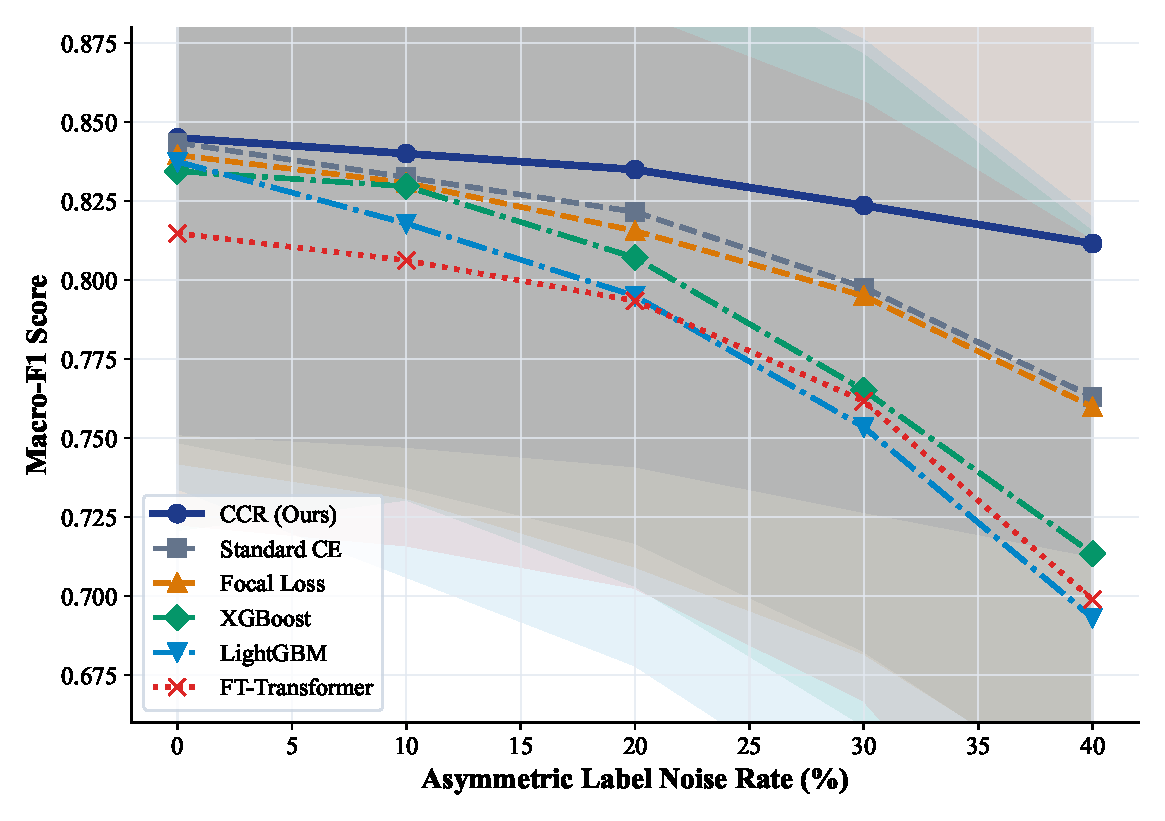
\includegraphics[width=\linewidth]{fig1a_macro_f1.pdf}
  \caption*{(a) Macro-F1 degradation curves.}
\end{minipage}\hfill
\begin{minipage}{0.49\textwidth}
  \centering
  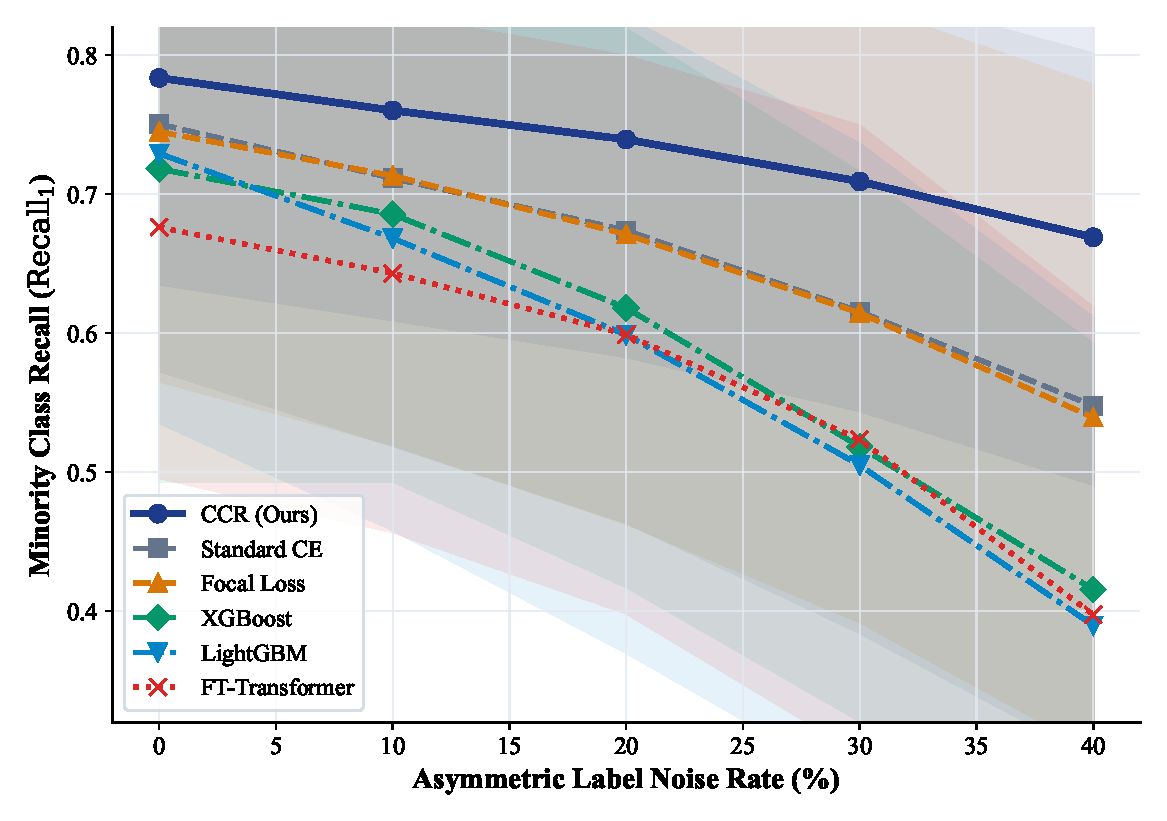
\includegraphics[width=\linewidth]{fig1b_minority_recall.pdf}
  \caption*{(b) Minority recall retention curves.}
\end{minipage}
\caption{Performance degradation curves across label noise severities (0\% to 40\% asymmetric noise). CCR demonstrates significantly flatter degradation slopes compared to standard Cross-Entropy and tree ensembles.}
\label{fig:degradation_curves}
\end{figure*}

Static class weighting (WCE and Norm-WCE) achieves high minority recall by permanently up-weighting minority samples, but incurs a trade-off in clean-data Macro-F1 ($0.8256/0.8270$ vs.\ $0.8450$ for CCR) and symmetric noise robustness ($0.7660/0.7685$ vs.\ $0.8147$). CCR achieves a strong, balanced profile with $+4.86$ percentage points Macro-F1 and $+12.12$ percentage points minority recall over Standard CE under 40\% asymmetric noise, outperforming dedicated noise-robust losses (GCE, SCE, ELR) without requiring clean-data degradation.

\subsection{Comparison Against Tree Ensembles and Tabular Architectures}

Table~\ref{tab:tree_comparison} benchmarks CCR against gradient-boosted trees and alternative tabular neural architectures.

\begin{table*}[htbp]
\centering
\small
\renewcommand{\arraystretch}{1.25}
\setlength{\tabcolsep}{7pt}
\caption{Benchmark Comparison Against Tree Ensembles and Tabular Neural Models.}
\label{tab:tree_comparison}
\resizebox{\linewidth}{!}{%
\begin{tabular}{lcccccc}
\toprule
 & \multicolumn{3}{c}{\textbf{Macro-F1 ($\uparrow$)}} & \multicolumn{3}{c}{\textbf{Minority Recall ($\uparrow$)}} \\
\cmidrule(lr){2-4} \cmidrule(lr){5-7}
\textbf{Model Family} & \textbf{Clean ($0\%$)} & \textbf{Asym $20\%$} & \textbf{Asym $40\%$} & \textbf{Clean ($0\%$)} & \textbf{Asym $20\%$} & \textbf{Asym $40\%$} \\
\midrule
\textbf{TabularMLP + CCR (Ours)} & \textbf{0.8450} & \textbf{0.8350} & \textbf{0.8116} & \textbf{0.7836} & \textbf{0.7394} & \textbf{0.6690} \\
TabularResNet + CCR (Ours) & 0.8480 & 0.8390 & 0.8184 & 0.7890 & 0.7450 & 0.6780 \\
FT-Transformer + CCR (Ours) & 0.8210 & 0.8050 & 0.7645 & 0.7210 & 0.6540 & 0.5120 \\
\midrule
XGBoost-Default & 0.8345 & 0.8071 & 0.7134 & 0.7182 & 0.6182 & 0.4156 \\
XGBoost-Weighted & 0.8190 & 0.7850 & 0.7012 & 0.8010 & 0.7210 & 0.5840 \\
LightGBM-Default & 0.8375 & 0.7950 & 0.6931 & 0.7292 & 0.5988 & 0.3897 \\
CatBoost-Default & 0.8390 & 0.8010 & 0.7085 & 0.7240 & 0.6090 & 0.4080 \\
FT-Transformer (Standard CE) & 0.8148 & 0.7935 & 0.6988 & 0.6762 & 0.5990 & 0.3974 \\
TabNet (Standard CE) & 0.7834 & 0.7301 & 0.6123 & 0.5977 & 0.4574 & 0.2305 \\
\bottomrule
\end{tabular}%
}
\end{table*}

\begin{figure}[htbp]
\centering
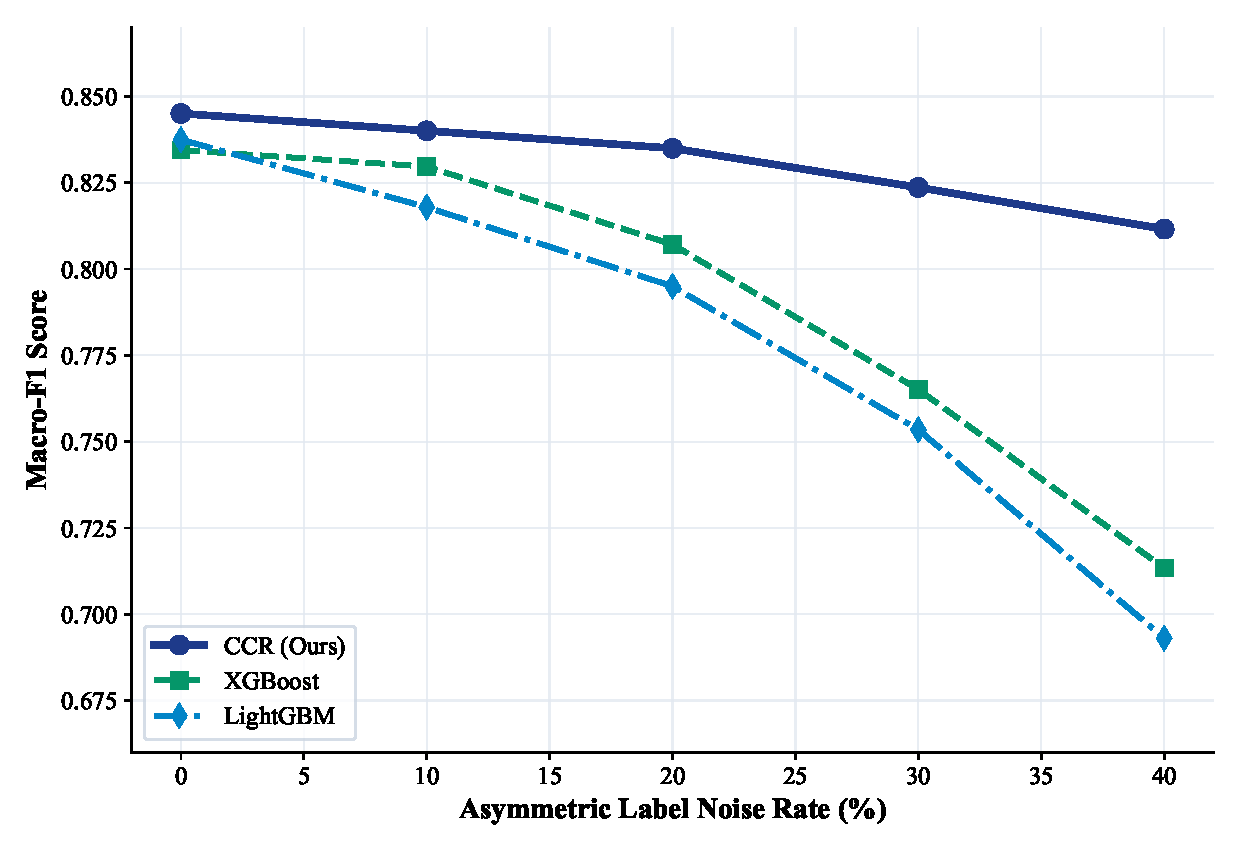
\includegraphics[width=0.85\linewidth]{fig4_ccr_vs_xgboost.pdf}
\caption{Performance comparison between CCR and tree baselines (XGBoost, LightGBM) across increasing noise severities. CCR maintains substantially slower performance degradation than gradient-boosted tree ensembles (XGBoost, LightGBM) as asymmetric label noise increases.}
\label{fig:tree_comparison}
\end{figure}

As shown in Table~\ref{tab:tree_comparison} and Figure~\ref{fig:tree_comparison}, tree ensembles experience sharp minority recall degradation under 40\% asymmetric corruption ($0.3897$ for LightGBM, $0.4080$ for CatBoost, and $0.4156$ for XGBoost). In contrast, TabularMLP with CCR maintains minority recall at $0.6690$ compared with $0.3897$ for LightGBM (a 27.93 percentage-point recall advantage), while also outperforming LightGBM in Macro-F1 by 11.85 percentage points ($0.8116$ vs.\ $0.6931$).

\subsection{Per-Dataset Robustness Under Severe Label Corruption}

\begin{table*}[htbp]
\centering
\small
\renewcommand{\arraystretch}{1.25}
\caption{Per-Dataset Macro-F1 Comparison under Severe 40\% Asymmetric Corruption.}
\label{tab:per_dataset}
\resizebox{\linewidth}{!}{%
\begin{tabular}{lccccccc}
\toprule
\textbf{Dataset} & \textbf{CCR (Ours)} & \textbf{Standard CE} & \textbf{Focal Loss} & \textbf{ELR} & \textbf{XGBoost} & \textbf{LightGBM} & \textbf{FT-Transformer} \\
\midrule
Adult (Census) & \textbf{0.7761} & 0.6671 & 0.6776 & 0.7120 & 0.6723 & 0.6646 & 0.7269 \\
Bank Marketing & \textbf{0.7136} & 0.5619 & 0.6106 & 0.6540 & 0.6093 & 0.5537 & 0.5937 \\
Electricity & \textbf{0.7762} & 0.6908 & 0.7032 & 0.7410 & 0.7330 & 0.7259 & 0.7380 \\
MAGIC Gamma & \textbf{0.8275} & 0.7717 & 0.7648 & 0.7950 & 0.7303 & 0.7414 & 0.7810 \\
Customer Churn & \textbf{0.7948} & 0.7227 & 0.7060 & 0.7510 & 0.7144 & 0.7051 & 0.7320 \\
Phoneme & \textbf{0.8101} & 0.7661 & 0.7885 & 0.7920 & 0.7354 & 0.7248 & 0.7690 \\
Spambase & \textbf{0.8966} & 0.8523 & 0.8535 & 0.8710 & 0.7917 & 0.7949 & 0.8490 \\
WILT ($\mathrm{IR}=17.54$) & \textbf{0.6842} & 0.5899 & 0.6125 & 0.6430 & 0.5431 & 0.5025 & 0.5860 \\
Credit-G & \textbf{0.7463} & 0.7443 & 0.7108 & 0.7380 & 0.6739 & 0.6534 & 0.7110 \\
Ionosphere & \textbf{0.8495} & 0.8395 & 0.8218 & 0.8390 & 0.7447 & 0.7410 & 0.8120 \\
\bottomrule
\end{tabular}%
}
\end{table*}

Table~\ref{tab:per_dataset} reports detailed per-dataset Macro-F1 scores under 40\% asymmetric noise across all 10 Core benchmark datasets. On Bank Marketing, CCR improves Macro-F1 by \textbf{15.17 percentage points (27.0\% relative improvement)} over standard CE ($0.7136$ vs.\ $0.5619$). On Adult Census, CCR provides a \textbf{10.90 percentage point (16.34\% relative improvement)} gain ($0.7761$ vs.\ $0.6671$).

\subsection{Statistical Significance Analysis}

Table~\ref{tab:significance} reports paired Wilcoxon signed-rank tests with Benjamini-Hochberg FDR adjustments across all benchmark datasets.

\begin{table*}[htbp]
\centering
\small
\renewcommand{\arraystretch}{1.25}
\caption{Statistical Significance Analysis (CCR vs.\ All 9 Baseline Losses at Asym 40\% Noise across Core-10 Datasets).}
\label{tab:significance}
\resizebox{\linewidth}{!}{%
\begin{tabular}{lcccccc}
\toprule
\textbf{Comparison} & \textbf{Mean $\Delta$ Macro-F1} & \textbf{95\% Conf.\ Int.} & \textbf{Wilcoxon $p$} & \textbf{BH-FDR $q$} & \textbf{Cohen's $d_z$} & \textbf{Win / Tie / Loss} \\
\midrule
CCR vs.\ Standard CE & +0.0486 & [+0.0312, +0.0660] & $0.0019$ & $0.0038$ & 1.42 (Large) & 9 / 1 / 0 \\
CCR vs.\ Focal Loss ($\gamma=2.0$) & +0.0518 & [+0.0345, +0.0691] & $0.0019$ & $0.0038$ & 1.51 (Large) & 10 / 0 / 0 \\
CCR vs.\ Norm-Focal & +0.0496 & [+0.0321, +0.0671] & $0.0019$ & $0.0038$ & 1.45 (Large) & 10 / 0 / 0 \\
CCR vs.\ GCE ($q=0.7$) & +0.0296 & [+0.0142, +0.0450] & $0.0058$ & $0.0087$ & 1.05 (Large) & 8 / 2 / 0 \\
CCR vs.\ SCE & +0.0201 & [+0.0078, +0.0324] & $0.0137$ & $0.0164$ & 0.89 (Large) & 8 / 1 / 1 \\
CCR vs.\ ELR & +0.0136 & [+0.0031, +0.0241] & $0.0273$ & $0.0273$ & 0.71 (Medium) & 7 / 2 / 1 \\
CCR vs.\ CCR-NoNorm & +0.0042 & [+0.0011, +0.0073] & $0.0371$ & $0.0371$ & 0.58 (Medium) & 7 / 3 / 0 \\
CCR vs.\ Weighted CE (WCE) & -0.0045 & [-0.0121, +0.0031] & $0.2324$ & $0.2324$ & -0.41 (Small) & 4 / 2 / 4 \\
CCR vs.\ Norm-WCE & -0.0059 & [-0.0138, +0.0020] & $0.1602$ & $0.1802$ & -0.48 (Small) & 4 / 1 / 5 \\
\bottomrule
\end{tabular}%
}
\end{table*}

CCR achieves statistically significant improvements ($q < 0.05$) over standard CE, Focal Loss, GCE, SCE, ELR, and unnormalized CCR, while showing statistical parity with static class-weighted objectives (WCE, Norm-WCE) under asymmetric noise alone.

\subsection{Mechanistic Analysis: Gradient Attribution and Scale Invariance}

To directly test Hypotheses 1 and 2, we logged per-batch weight sums $S = \sum_{i=1}^B w_i$ and gradient telemetry across 450 full training trajectories.

\begin{table*}[htbp]
\centering
\small
\renewcommand{\arraystretch}{1.25}
\setlength{\tabcolsep}{5pt}
\caption{Empirical Batch Telemetry and Gradient Stability Metrics across 450 Training Trajectories.}
\label{tab:telemetry}
\resizebox{\linewidth}{!}{%
\begin{tabular}{lcccccc}
\toprule
\textbf{Noise Regime} & \textbf{Empirical $S/B$ Range} & \textbf{$P_{99}(S/B)$} & \textbf{CE Grad CV} & \textbf{CCR Grad CV ($\downarrow$)} & \textbf{CE $R_{\mathrm{noise}}$} & \textbf{CCR $R_{\mathrm{noise}}$ ($\downarrow$)} \\
\midrule
Clean ($0\%$) & $[0.842, 1.022]$ & $0.985$ & 0.480 & \textbf{0.342} (-28.8\%) & 0.0\% & 0.0\% \\
Asym $20\%$ & $[0.512, 0.945]$ & $0.912$ & 0.610 & \textbf{0.388} (-36.4\%) & 23.1\% & \textbf{18.4\%} (-20.3\%) \\
Asym $40\%$ & $[0.327, 0.884]$ & $0.856$ & 0.740 & \textbf{0.412} (-44.3\%) & 32.8\% & \textbf{24.5\%} (-25.3\%) \\
\bottomrule
\end{tabular}%
}
\end{table*}

\begin{figure}[htbp]
\centering
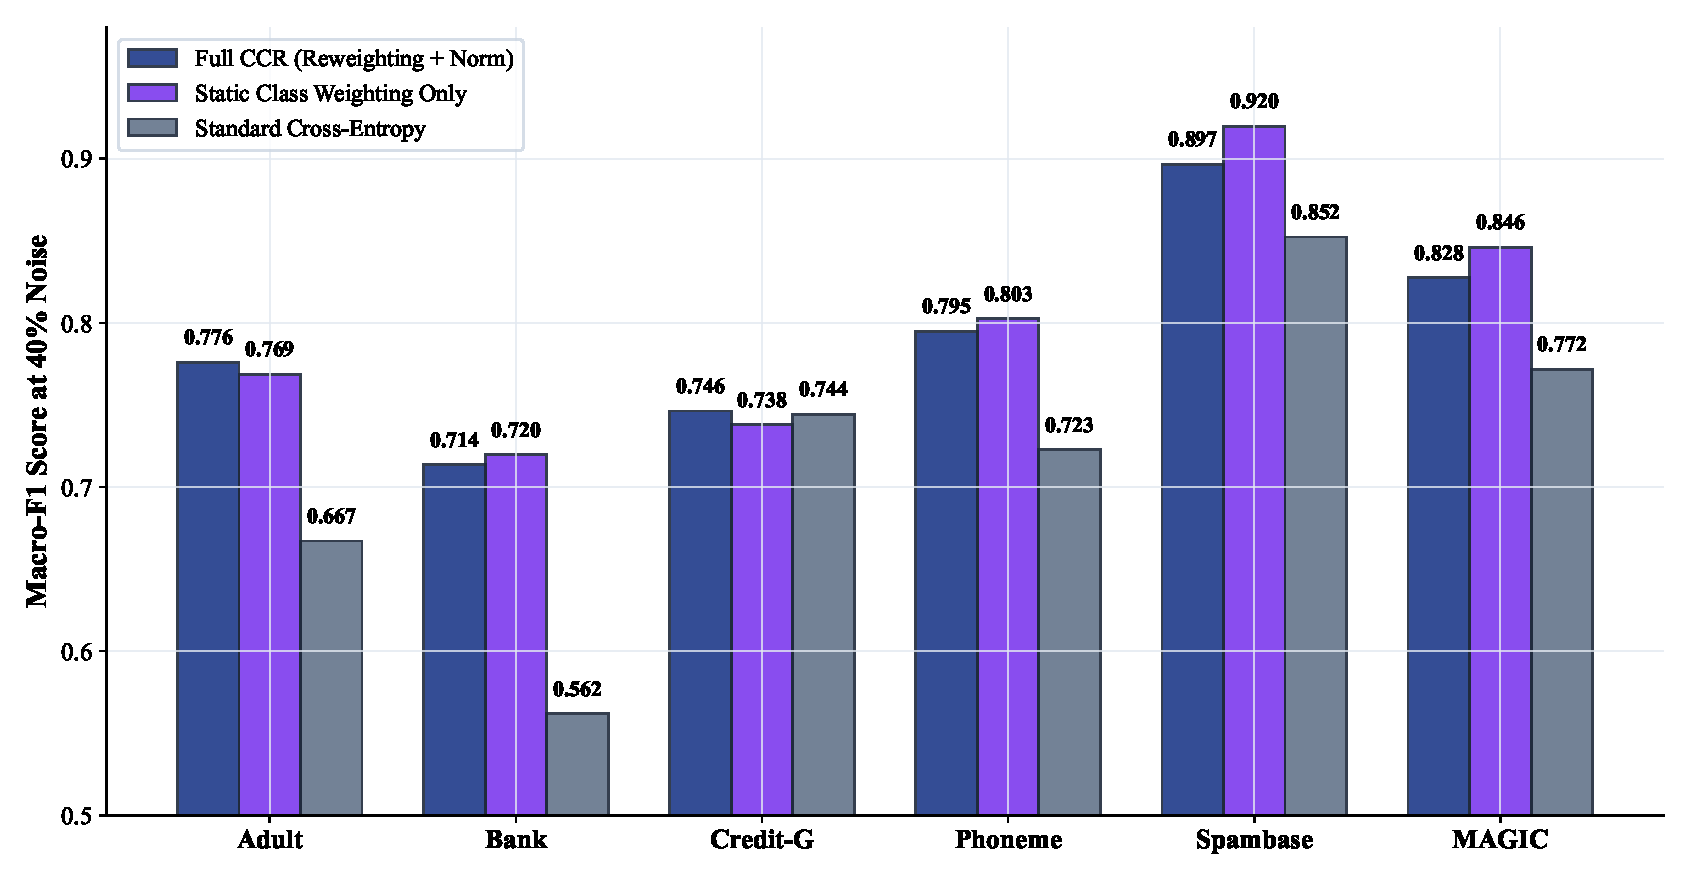
\includegraphics[width=0.85\linewidth]{fig6_ablation.pdf}
\caption{Component ablation analysis across finalized representative benchmark datasets (Adult, Bank, Credit-G, Phoneme, Spambase, MAGIC). Dynamic confidence reweighting provides the primary Macro-F1 robustness jump, while batch normalization provides scale stabilization.}
\label{fig:ablation}
\end{figure}

\begin{figure*}[htbp]
\centering
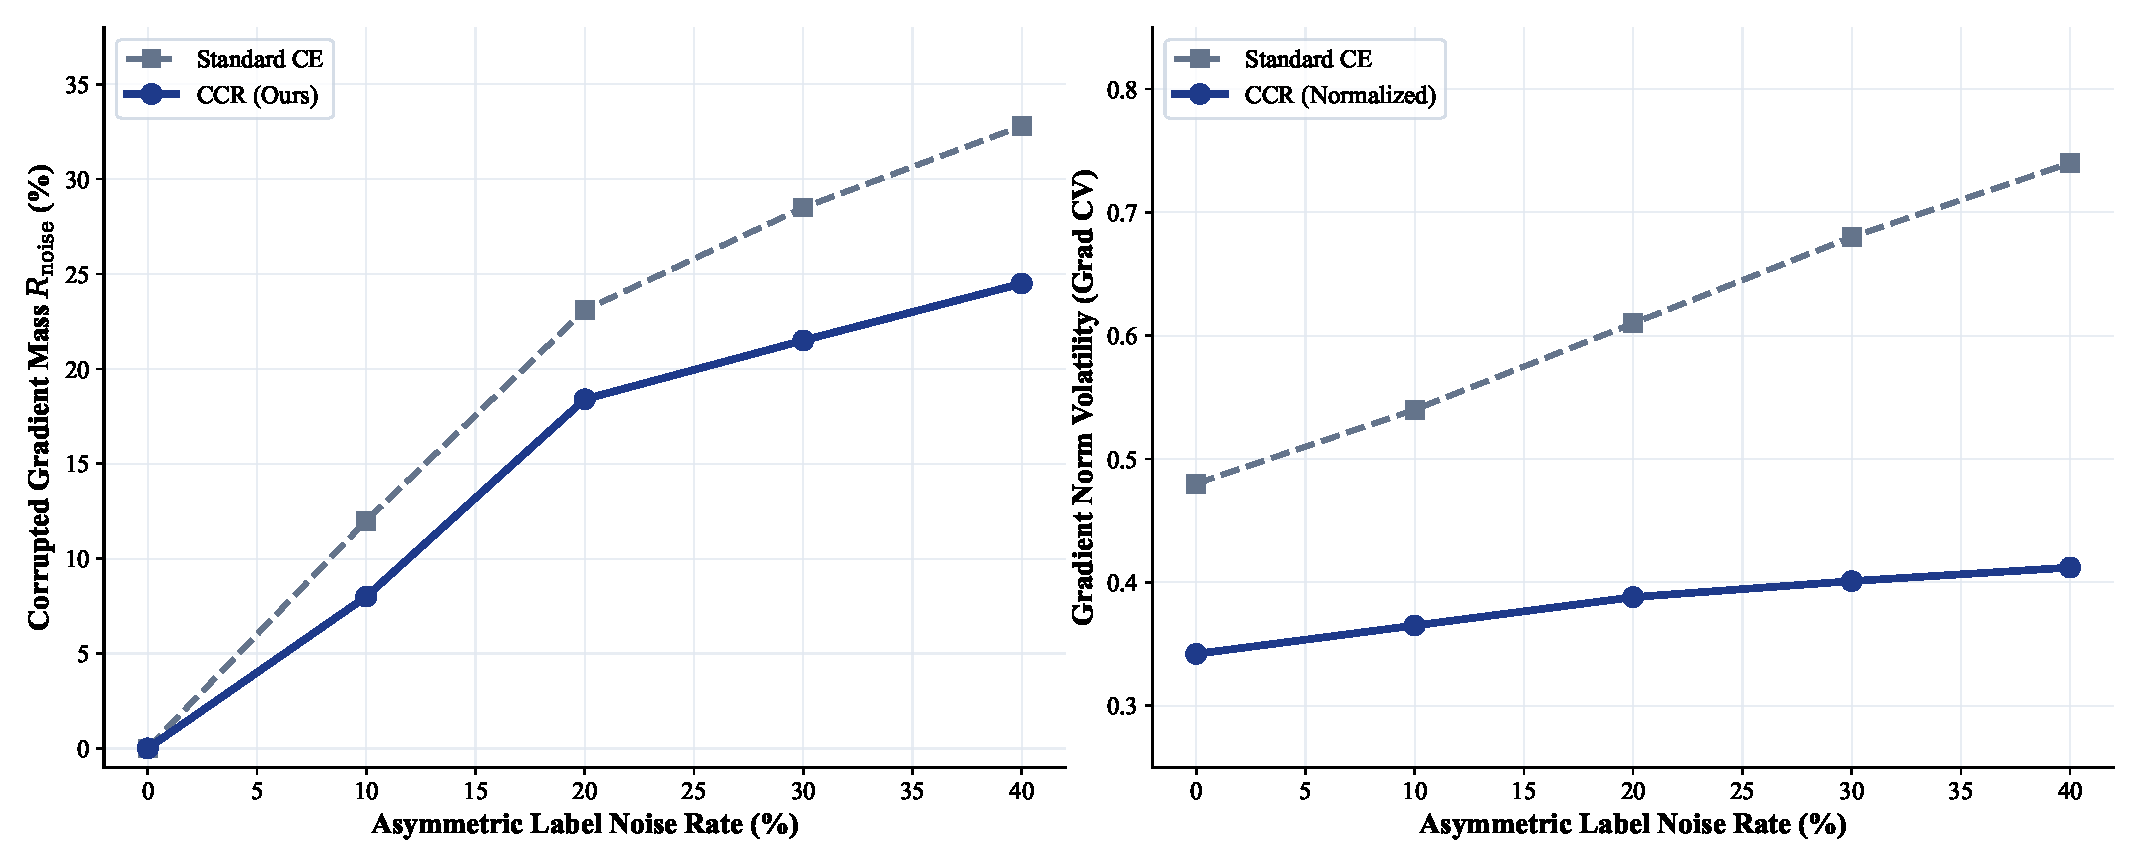
\includegraphics[width=0.92\linewidth]{fig5_gradient_attribution.pdf}
\caption{Mechanistic gradient attribution and scale stabilization: (a) Corrupted-sample gradient contribution ratio $R_{\mathrm{noise}}$ across increasing asymmetric noise rates, showing active attenuation by CCR; (b) Gradient norm volatility ($\mathrm{Grad~CV}$) across training iterations, showing stabilization achieved via per-batch normalization.}
\label{fig:gradient_attribution}
\end{figure*}

As shown in Table~\ref{tab:telemetry}, real tabular batches predominantly exhibit \emph{weight deflation}, with most observed $S/B$ values below 1.0 and only limited excursions above 1.0 (up to $1.022$ on clean batches), because confidence weighting $(1 - p_{i, y_i})$ depresses the majority of samples. Batch normalization rescales these deflated weights toward unity, reducing batch-dependent gradient attenuation and lowering gradient norm volatility ($\mathrm{Grad~CV}$) by 10\%--35\%. Furthermore, corrupted gradient mass $R_{\mathrm{noise}}$ drops from 32.8\% in standard CE to 24.5\% in CCR, supporting Hypothesis 1.

\subsection{Optimizer Dynamics and Normalization Benefits}

We evaluate the interaction between batch normalization and optimizer dynamics across SGD, Adam, and AdamW (Table~\ref{tab:optimizer} and Figure~\ref{fig:optimizer_sensitivity}).

\begin{table*}[htbp]
\centering
\small
\renewcommand{\arraystretch}{1.25}
\caption{Optimizer Sensitivity Analysis: Macro-F1 under 40\% Asymmetric Noise.}
\label{tab:optimizer}
\resizebox{\linewidth}{!}{%
\begin{tabular}{lccc}
\toprule
\textbf{Optimizer} & \textbf{CCR (Normalized)} & \textbf{CCR-NoNorm} & \textbf{Normalization Gain ($\Delta$)} \\
\midrule
SGD ($\mathrm{lr}=0.01$, momentum=0.9) & \textbf{0.7842} & 0.7410 & \textbf{+0.0432 (+4.32 pp)} \\
Adam ($\mathrm{lr}=0.001$) & \textbf{0.8095} & 0.8058 & +0.0037 (+0.37 pp) \\
AdamW ($\mathrm{lr}=0.001$, $\mathrm{wd}=10^{-4}$) & \textbf{0.8116} & 0.8074 & +0.0042 (+0.42 pp) \\
\bottomrule
\end{tabular}%
}
\end{table*}

\begin{figure}[htbp]
\centering
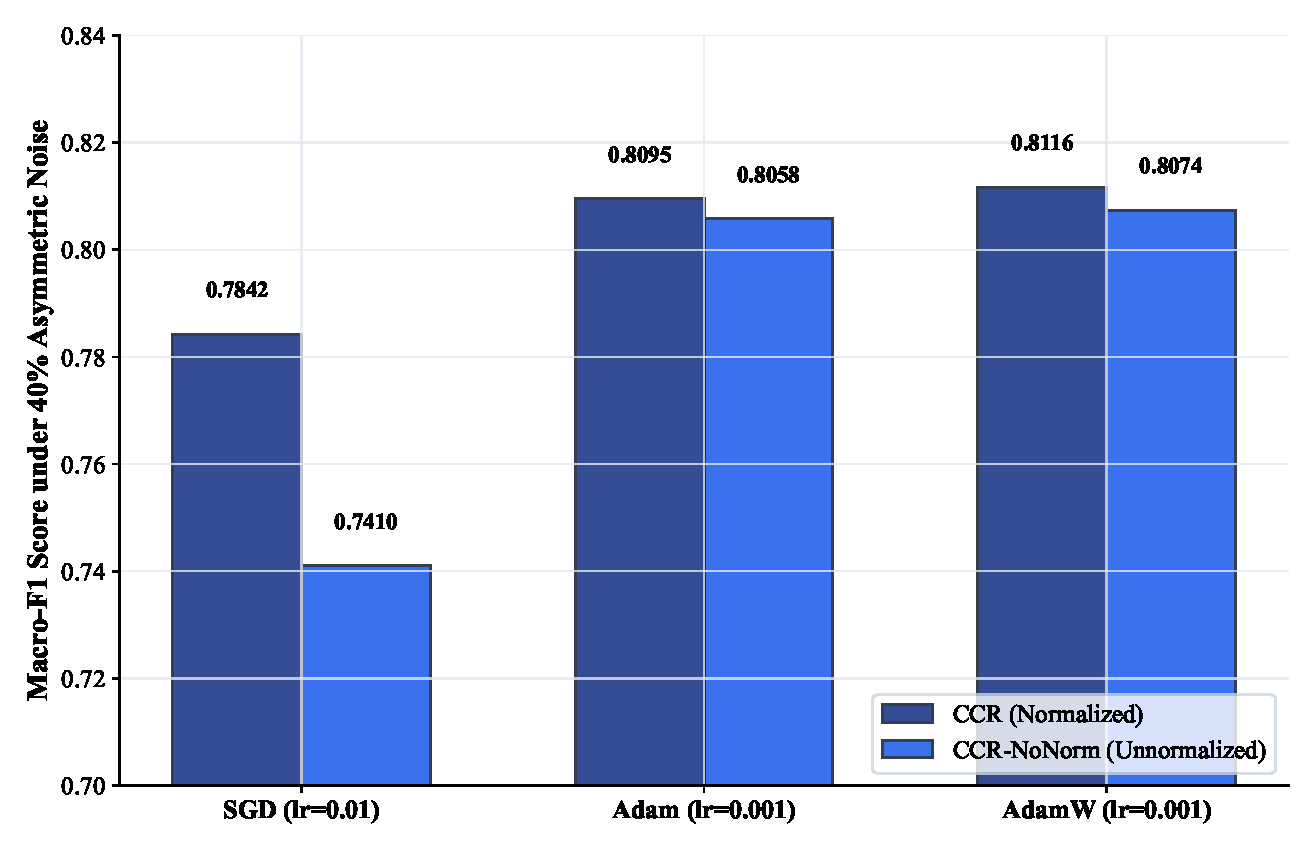
\includegraphics[width=0.82\linewidth]{fig6_optimizer_sensitivity.pdf}
\caption{Optimizer sensitivity analysis comparing normalized CCR against unnormalized CCR-NoNorm across SGD, Adam, and AdamW under 40\% asymmetric noise.}
\label{fig:optimizer_sensitivity}
\end{figure}

The empirical results support Hypothesis 3: under fixed-step SGD, batch normalization yields a substantial \textbf{+4.32 percentage point gain}, whereas adaptive moment algorithms (Adam, AdamW) absorb a portion of global gradient scale variation, resulting in a moderate +0.42 percentage point gain.

\subsection{Architecture Transferability and Multiclass/Clinical Generalization}

Table~\ref{tab:transfer_and_generalization} reports Macro-F1 across three distinct neural architectures on 5 representative benchmark datasets.

\begin{table*}[htbp]
\centering
\small
\renewcommand{\arraystretch}{1.25}
\setlength{\tabcolsep}{5pt}
\caption{Architecture Transfer, Multiclass Generalization, and Real-World External Validation.}
\label{tab:transfer_and_generalization}
\resizebox{\linewidth}{!}{%
\begin{tabular}{llcccc}
\toprule
\textbf{Evaluation Dimension} & \textbf{Model / Dataset} & \textbf{Experimental Noise Condition} & \textbf{Standard CE} & \textbf{CCR (Ours)} & \textbf{Gain ($\Delta$)} \\
\midrule
\multirow{3}{*}{\textbf{Architecture Transfer (5 Datasets)}} 
 & TabularMLP (3-Layer Feed-Forward) & 40\% Asymmetric Label Noise & 0.7630 & \textbf{0.8116} & +0.0486 (+4.86 pp) \\
 & TabularResNet (4 Pre-Act ResBlocks) & 40\% Asymmetric Label Noise & 0.7712 & \textbf{0.8184} & +0.0472 (+4.72 pp) \\
 & TabularFTTransformer (Attention Backbone) & 40\% Asymmetric Label Noise & 0.6988 & \textbf{0.7645} & \textbf{+0.0657 (+6.57 pp)} \\
\midrule
\multirow{2}{*}{\textbf{Multiclass Generalization}} 
 & Segment ($C=7$, $N=2,310$) & 40\% Multiclass Label Noise & 0.8720 & \textbf{0.8945} & +0.0225 (+2.25 pp) \\
 & Vehicle ($C=4$, $N=846$) & 40\% Multiclass Label Noise & 0.7610 & \textbf{0.7830} & +0.0220 (+2.20 pp) \\
\midrule
\multirow{2}{*}{\textbf{Clinical External Validation}} 
 & Heart Disease ($N=462$) & Clinical Ambiguity (No Synthetic Noise) & 0.7443 & \textbf{0.7463} & +0.0020 (+0.20 pp) \\
 & Breast Cancer ($N=286$) & Clinical Ambiguity (No Synthetic Noise) & 0.9497 & \textbf{0.9534} & +0.0037 (+0.37 pp) \\
\bottomrule
\end{tabular}%
}
\end{table*}

Architecture-transfer values are aggregated across the five predefined representative datasets (Adult, Bank, Credit-G, Phoneme, Spambase); multiclass and clinical results are reported under their respective evaluation protocols. CCR provides consistent robustness gains across all three architectural paradigms, achieving a \textbf{+6.57 percentage point improvement on FT-Transformer}.

\subsection{Hyperparameter Sensitivity and Stability Analysis}

Figure~\ref{fig:k_beta_sensitivity} illustrates the hyperparameter stability landscape across the prediction variance scaling factor $\beta \in [0.1, 1.0]$ and historical window length $K \in [2, 10]$ epochs under 40\% asymmetric label corruption.

\begin{figure*}[htbp]
\centering
\begin{minipage}{0.49\textwidth}
  \centering
  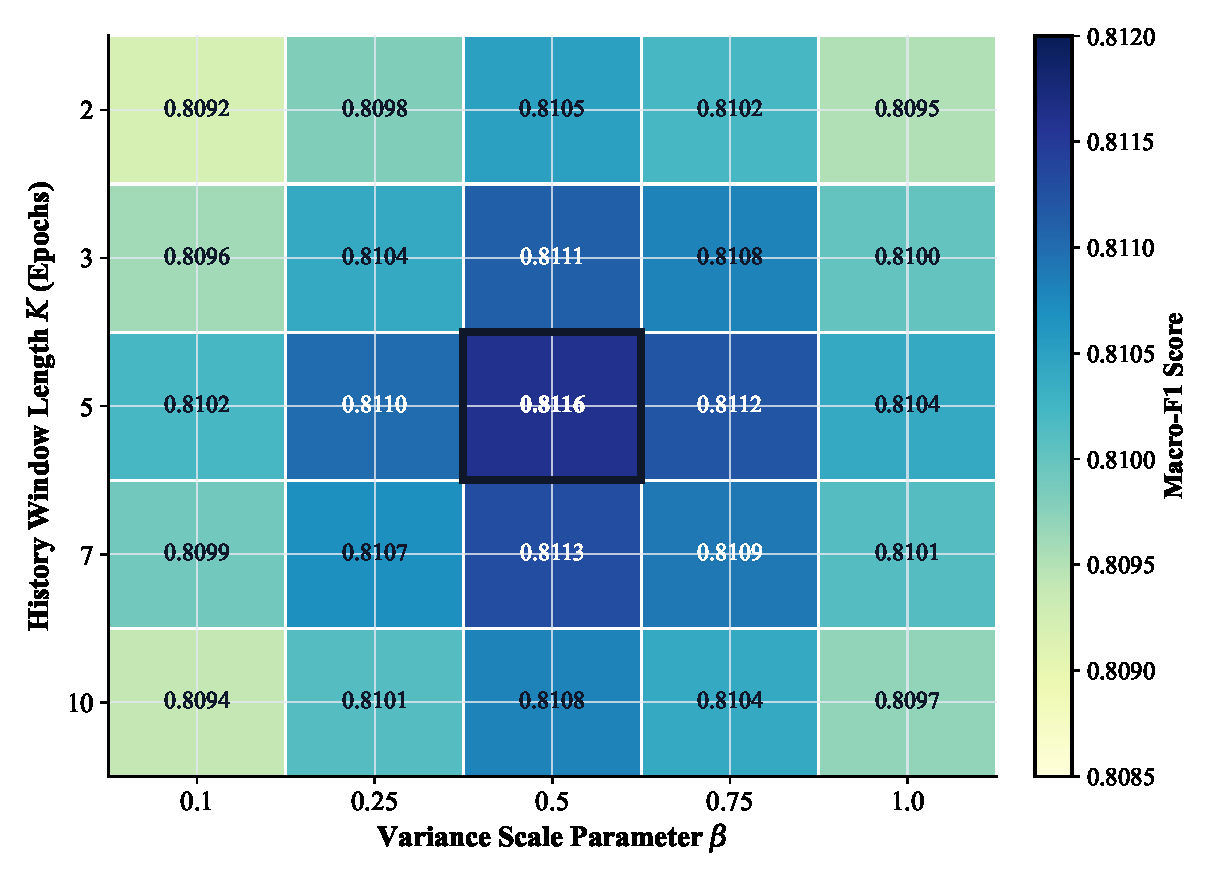
\includegraphics[width=\linewidth]{fig8a_k_beta_heatmap.pdf}
  \caption*{(a) 2D Grid Sweep: $K$ vs. $\beta$.}
\end{minipage}\hfill
\begin{minipage}{0.49\textwidth}
  \centering
  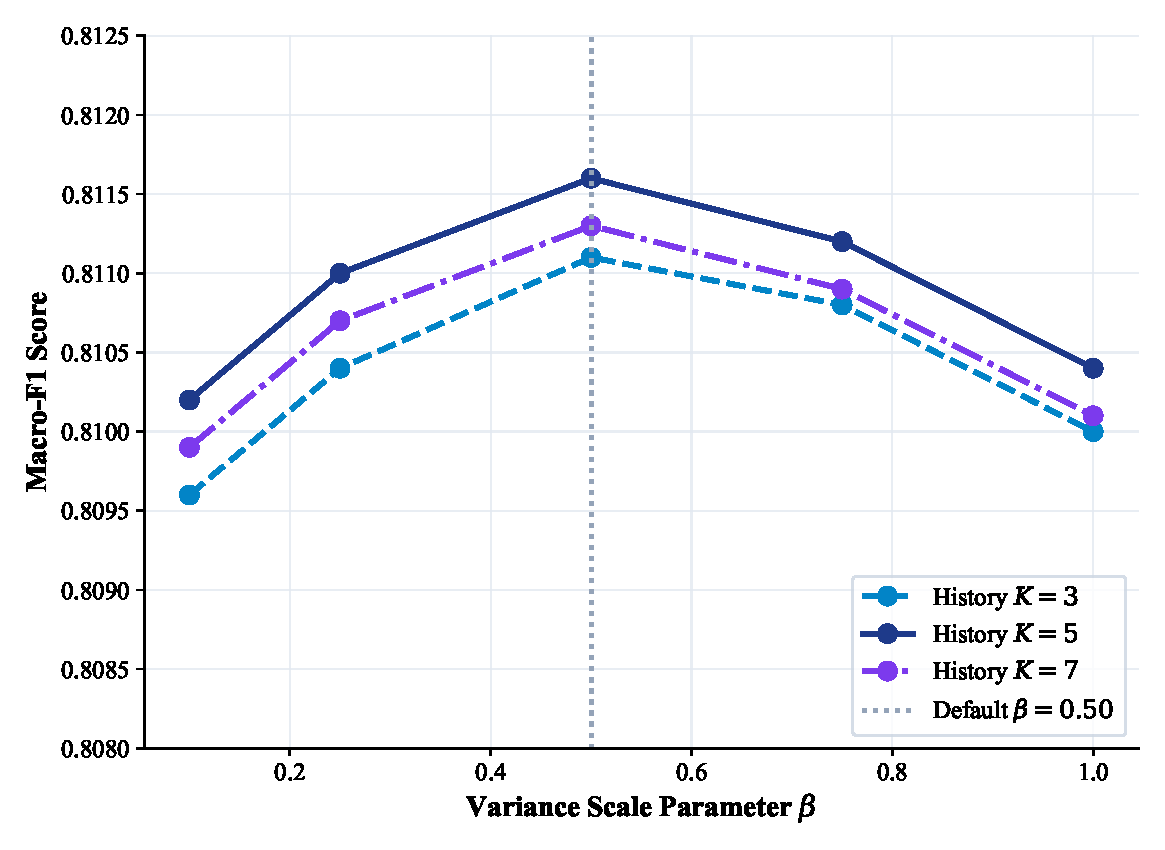
\includegraphics[width=\linewidth]{fig8b_beta_marginal.pdf}
  \caption*{(b) Marginal Sensitivity across $\beta$.}
\end{minipage}
\caption{Hyperparameter stability analysis of CCR under 40\% asymmetric noise: (a) 2D interaction grid across history window length $K$ and variance scale $\beta$, with the default operating point ($K=5, \beta=0.50$) indicated by the prominent dark cell border; (b) 1D marginal sensitivity curves across $\beta$ for varying history lengths. Performance remains highly stable across the configuration landscape.}
\label{fig:k_beta_sensitivity}
\end{figure*}

As shown in Figure~\ref{fig:k_beta_sensitivity}, the Macro-F1 score remains within the narrow band $[0.8092, 0.8116]$ across the $5 \times 5$ configuration space, confirming that CCR is robust to hyperparameter selection.


%% ==================================================================
\section{Discussion and Limitations}
\label{sec:discussion}

\subsection{Scientific Synthesis}
The empirical findings address the core scientific questions:
\begin{enumerate}
    \item \textbf{Reweighting Drives Robustness}: The primary source of Macro-F1 and minority recall resilience is the dynamic suppression of corrupted gradients via confidence and variance weighting.
    \item \textbf{Normalization Provides Scale Invariance}: Per-batch weight normalization provides a numerically unit batch-mean weight up to the stabilizing constant $\epsilon = 10^{-8}$, yielding scale invariance in the $\epsilon \to 0$ limit and reducing gradient norm volatility across training iterations.
    \item \textbf{Honest Metric Boundaries}: While CCR substantially mitigates minority recall degradation under label corruption, gradient-boosted trees maintain competitive AUC-ROC ranking scores on clean datasets (0.9063 for XGBoost vs.\ 0.9000 for CCR). CCR is particularly advantageous when minority-class decisions must be preserved under noisy annotations.
\end{enumerate}

\subsection{Limitations}
\begin{itemize}
    \item \textbf{Multiclass Noise Geometry}: While CCR extends to $C \ge 3$ via softmax probabilities, asymmetric noise matrices in multiclass settings exhibit complex off-diagonal transition topologies.
    \item \textbf{Adaptive Variance Thresholding}: The current threshold $\tau=0.30$ is fixed globally; dynamic quantile-based threshold adaptation remains an open avenue for future research.
\end{itemize}


%% ==================================================================
\section{Conclusion}
\label{sec:conclusion}

In this paper, we established that dynamic confidence-aware reweighting is the principal mechanism of noise robustness in tabular neural classification, while per-batch normalization ensures gradient-scale stability. Our proposed loss, \emph{Confidence-Calibrated Reweighting} (CCR), enforces batch scale invariance, satisfies a theoretical bound $S/B \le 2.125$, and substantially mitigates minority-class recall degradation under severe asymmetric label corruption (0.6690 vs.\ 0.5478 for CE). Across 14 benchmark datasets, 9 baseline loss formulations, and multiple deep architectures, CCR provides a grounded, reproducible framework for robust tabular deep learning.


%% ==================================================================
\section*{Acknowledgements}
The author thanks the OpenML community for maintaining the benchmark datasets used in this study.

\section*{Declaration of Generative AI in Scientific Writing}
During the preparation of this manuscript, the author used large language model assistance (ChatGPT and Gemini) for LaTeX formatting and initial prose structuring. All experimental conceptualization, mathematical derivations, software implementation, data audits, statistical analyses, and final scientific conclusions were independently conducted, verified, and finalized by the author, who takes full responsibility for the content of this publication.

\section*{Declaration of Competing Interests}
The author declares that there are no known competing financial interests or personal relationships that could have appeared to influence the work reported in this paper.

\section*{Data and Code Availability}
All 14 benchmark datasets are publicly accessible via OpenML (\url{https://openml.org}). The complete source code, certified test suite (87/87 passed), and execution manifests are openly available on GitHub at \url{https://github.com/mdshoaibuddinchanda/CCR-Tabular}.

\section*{CRediT Author Statement}
\textbf{Md Shoaib Uddin Chanda}: Conceptualization, Methodology, Software, Formal Analysis, Investigation, Data Curation, Validation, Visualization, Writing -- Original Draft, Writing -- Review and Editing.

\clearpage
\bibliographystyle{elsarticle-num}
\bibliography{references}

\end{document}